Prior we begin our discussion it is worth to introduce a few preliminary facts and statements.
Define the iterated rascal number
\begin{definition}
    Iterated rascal number
    \begin{align}
        \rascalNumber{n}{k}{i} = \sum_{m=0}^{i} \binom{n-k}{m} \binom{k}{m}
    \end{align}
\end{definition}
The first important thing to notice is that the iterated Rascal number is a special case of the Vandermonde convolution.
Consider the Vandermonde convolution~\cite{andrews1999special}
\begin{equation*}
    \binom{a+b}{r} = \sum_{m=0}^{r} \binom{a}{m} \binom{b}{r-m}; \quad \binom{n}{k} = \sum_{m=0}^{k} \binom{n-k}{m} \binom{k}{k-m}
\end{equation*}
Thus,
\begin{equation}
    \rascalNumber{n}{k}{i} = \sum_{m=0}^{i} \binom{n-k}{m} \binom{k}{k-m}
    \label{eq:rascal-vandermonde-convolution}
\end{equation}
Meaning that iterated rascal number is partial case of Vandermonde convolution of $\binom{n}{k}$
with the upper summation bound equals to $i$.
Without further hesitation consider our findings.
\begin{proposition}
    \label{prop:rascal-binomial-identity-for-i}
    Iterated rascal triangle equals to Pascal's triangle up to $i$-th column.
    \begin{equation}
        \rascalNumber{n}{k}{i} = \binom{n}{k}, \quad 0 \leq k \leq i
        \label{eq:rascal-column-identity}
    \end{equation}
\end{proposition}
Then binomial identity follows
\begin{align*}
    \rascalNumber{n}{i-k}{i} = \binom{n}{i-k}
\end{align*}
Applying binomial coefficients symmetry principle we obtain
\begin{align*}
    \rascalNumber{n}{n-i+k}{i} = \binom{n}{n-i+k}
\end{align*}
\begin{proof}
    Proof of proposition~\eqref{prop:rascal-binomial-identity-for-i}.
    Consider the following relation between binomial coefficients and iterated rascal numbers,
    for every $0 \leq k \leq i$
    \begin{align*}
        \binom{n}{k} - \rascalNumber{n}{k}{i} &= \sum_{m=0}^{k} \binom{n-k}{m} \binom{k}{k-m} - \sum_{m=0}^{i} \binom{n-k}{m} \binom{k}{k-m} \\
        &=  \sum_{m=k+1}^{i} \binom{n-k}{m} \binom{k}{m} = 0
    \end{align*}
    It is indeed true, because binomial coefficients $\binom{k}{m}$ are zero for each $m \geq k+1$.
    So that for every $0 \leq k \leq i$
    \begin{align*}
        \binom{n}{k} - \rascalNumber{n}{k}{i} = 0; \quad \binom{n}{k} = \rascalNumber{n}{k}{i}
    \end{align*}
    Therefore, the proposition~\eqref{prop:rascal-binomial-identity-for-i} is true.
\end{proof}
\begin{proposition}
    \label{prop:odd-row-proposition}
    Iterated rascal triangle equals to Pascal's triangle up to $2i+1$-th row
    \begin{align*}
        \rascalNumber{n}{k}{i} = \binom{n}{k}, \quad 0 \leq n \leq 2i+1
    \end{align*}
\end{proposition}
Therefore, for every fixed $i \geq 0$ and $n \geq 0$
\begin{equation}
    \rascalNumber{2i+1-n}{k}{i} = \binom{2i+1-n}{k}
    \label{eq:odd-row-identity}
\end{equation}
Equation~\eqref{eq:odd-row-identity} is of interest because in contrast to rascal
column identity~\eqref{eq:rascal-column-identity} it gives relation over $k$ for each $i$,
so that it is true for all cases in $i,k$: $i < k$, $i=k$ and $k >i$.
In particular, equation~\eqref{eq:odd-row-identity} implies the row sums identity in iterated rascal triangles
\begin{align*}
    \sum_{k=0}^{\infty} \rascalNumber{2i+1-n}{k}{i} = 2^{2i+1-n}
\end{align*}
Given $n=0$ we obtain
\begin{align*}
    \sum_{k=0}^{\infty} \rascalNumber{2i+1}{k}{i} = 2^{2i+1}
\end{align*}
and so on.
Taking $t=2i+1$ in~\eqref{eq:odd-row-identity} yields
\begin{align*}
    \rascalNumber{t-n}{k}{t-i-1}= \binom{t-n}{k}
\end{align*}
Moreover, equation~\eqref{eq:odd-row-identity} gives Vandermonde-like identity
\begin{proposition} (Vandermonde-like identity.)
    \label{prop:vandermonde-like-identity}
    \begin{equation*}
        \binom{2i+1-n}{k} = \sum_{m=0}^{i} \binom{2i+1-n-k}{m} \binom{k}{m}
    \end{equation*}
\end{proposition}
In particular, given $n=0,1$ proposition~\eqref{prop:vandermonde-like-identity}
gives the following binomial identities
\begin{align*}
    \binom{2i+1}{k} &= \sum_{m=0}^{i} \binom{2i+1-k}{m} \binom{k}{m} \\
    \binom{2i}{k}   &= \sum_{m=0}^{i} \binom{2i-k}{m} \binom{k}{m}
\end{align*}
\begin{proof}
    Proof of proposition~\eqref{prop:odd-row-proposition}.
%    We have three possible relations between $i,k$: $k<i$, $k=i$, $k > i$.
    We have to prove that for every $i,k$
    \begin{equation*}
        \sum_{m=0}^{k} \binom{2i+1-n-k}{m} \binom{k}{m} - \sum_{m=0}^{i} \binom{2i+1-n-k}{m} \binom{k}{m} = 0
    \end{equation*}
    For the case $k<i$ proof is the same as proof of proposition~\eqref{prop:rascal-binomial-identity-for-i}.
    For the case $k=i$ proof is trivial.
    Thus, the remaining case is $k>i$ yields
    \begin{equation*}
        \sum_{m=i+1}^{k} \binom{2i+1-n-k}{m} \binom{k}{m} = 0
    \end{equation*}
    Introducing sum in $k$ to above equation
    \begin{equation*}
        \sum_{m=i+1}^{k} \sum_{k} \binom{2i+1-n-k}{m} \binom{k}{m} = 0
    \end{equation*}
    Implies
    \begin{equation*}
        \sum_{m=i+1}^{k} \binom{2i+2-n}{2m+1} = 0
    \end{equation*}
    because $\sum_{k=0}^{l} \binom{l-k}{m} \binom{q+k}{n} = \binom{l+q+1}{m+n+1}$, see equation (5.26) in~\cite{graham1994concrete}.
    Substituting $m=i+1+m$ we get
    \begin{equation*}
        \sum_{m=0}^{k} \binom{2i+2-n}{2(i+1+m)+1} = \sum_{m=0}^{k} \binom{2i+2-n}{2i+3+2m} = 0
    \end{equation*}
    Which is indeed true for every $m,n \geq 0$.
    This completes the proof.
\end{proof}

Now, let's smoothly switch our focus to finite differences of binomial coefficients and iterated rascal numbers.
Considering the table of differences $\binom{n}{k}-\rascalNumber{n}{k}{3}$
\begin{figure}[H]
    \centering
    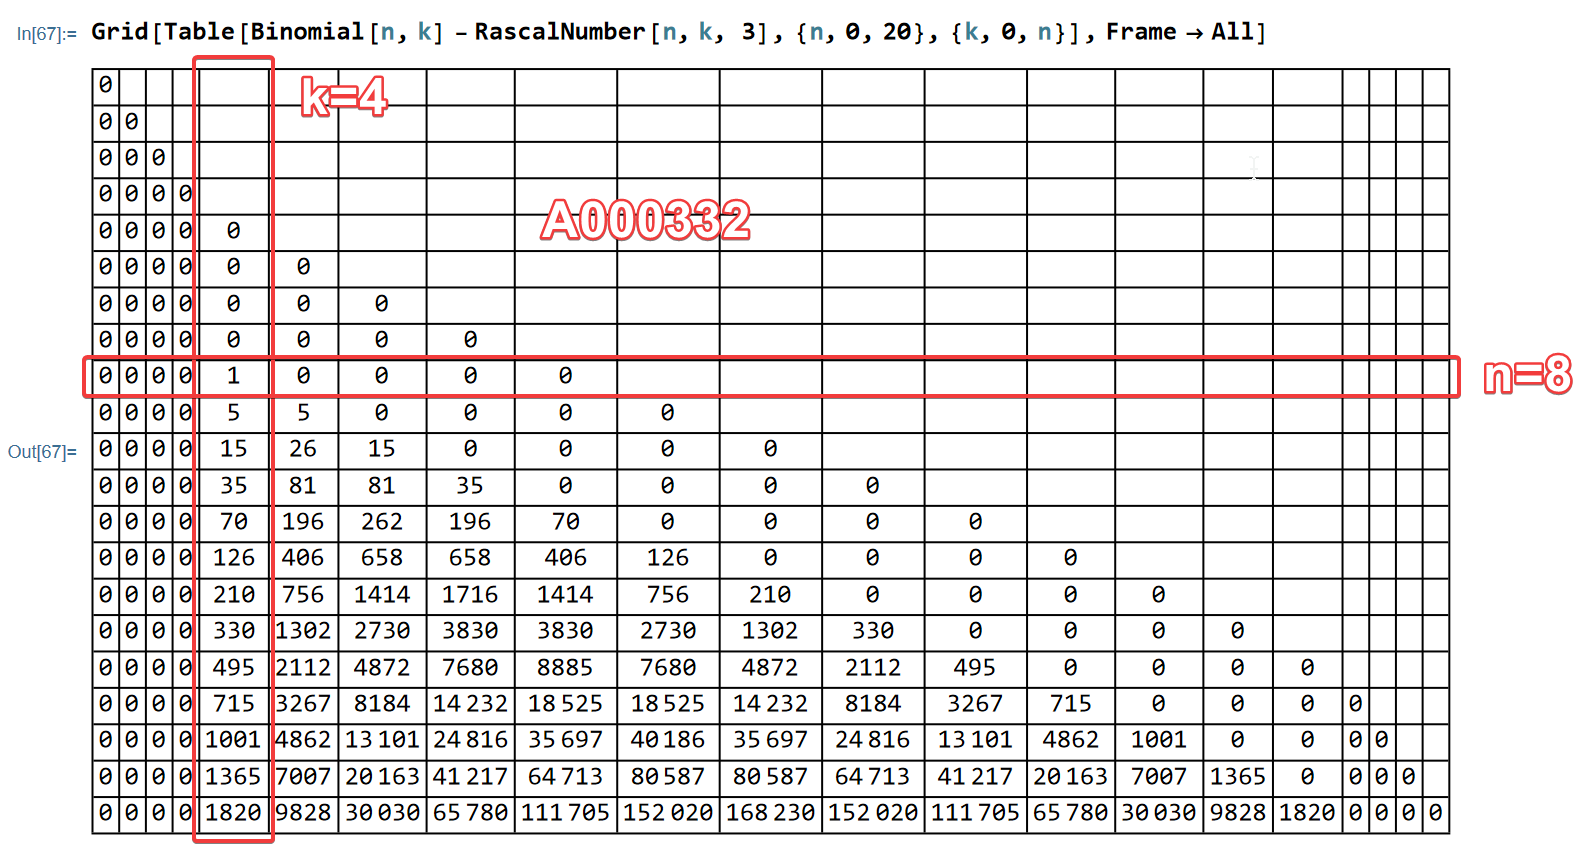
\includegraphics[width=1\textwidth]{img/01_Difference_Binomial_Rascal_i_3_BinomialCoefficients}
    ~\caption{Difference $\binom{n}{k}-\rascalNumber{n}{k}{3}$.
    Highlighted column is $\binom{n}{4}$.
    Sequence \href{https://oeis.org/A000332}{\texttt{A000332}} in the OEIS~\cite{sloane2009binomial}.}
    \label{fig:difference-binomial-rascal-i-3}
\end{figure}
We can spot that having $i=3$ the $k=4$-th column gives binomial coefficient $\binom{n}{4}$.
Indeed, this rule is true for every $i$.
\begin{proposition}
    \label{prop:row-column-difference}
    (Row-column difference.) For every fixed $i\geq0$
    \begin{align*}
        \binom{n+2i}{i} - \rascalNumber{n+2i}{i}{i-1} = \binom{n+i}{i}
    \end{align*}
    \begin{proof}
        We have previously stated that iterated rascal numbers are
        closely related to Vandermonde convolution~\eqref{eq:rascal-vandermonde-convolution}.
        Thus, proposition~\eqref{prop:row-column-difference} can be rewritten as
        \begin{align*}
            \sum_{m=0}^{i} \binom{n+i}{m} \binom{i}{i-m} - \sum_{m=0}^{i-1} \binom{n+i}{m} \binom{i}{i-m} = \binom{n+i}{i} \binom{i}{0}
        \end{align*}
        Therefore, $\binom{n+2i}{i} - \rascalNumber{n+2i}{i}{i-1} = \binom{n+i}{i}$ is indeed true.
    \end{proof}
\end{proposition}
Proposition~\eqref{prop:row-column-difference} yields to few more identities.
Applying binomial coefficients symmetry
\begin{align*}
    \binom{n+2i}{n+i} - \rascalNumber{n+2i}{n+i}{i-1} &= \binom{n+i}{n}
\end{align*}
Taking $j=n+i$ gives
\begin{align*}
    \binom{j+i}{j} - \rascalNumber{j+i}{j}{i-1} &= \binom{j}{j-i} \\
    \binom{j+i}{i} - \rascalNumber{j+i}{i}{i-1} &= \binom{j}{i}
\end{align*}
Proposition~\eqref{prop:row-column-difference} can be generalized even further, for every fixed $i<k$ and $i>k$.
\begin{proposition}
(Finite difference of binomial coefficients and iterated rascal numbers for $i<k$.)
    For every fixed $i<k$
    \label{prop:row-column-difference-general}
    \begin{align*}
        \binom{n}{k} - \rascalNumber{n}{k}{i} &= \sum_{m=i+1}^{k} \binom{n-k}{m} \binom{k}{k-m}
    \end{align*}
    \begin{proof}
        It is true by means of Vandermonde convolution.
    \end{proof}
\end{proposition}
\begin{proposition}
(Finite difference of binomial coefficients and iterated rascal numbers for $i>k$.)
    For every fixed $i>k$
    \label{prop:row-column-difference-general-i-greater-k}
    \begin{align*}
        \binom{n}{k} - \rascalNumber{n}{k}{i} &= \sum_{m=k+1}^{i} \binom{n-k}{m} \binom{k}{k-m}
    \end{align*}
    \begin{proof}
        It is true by means of Vandermonde convolution.
    \end{proof}
\end{proposition}
